\chapter[Plano de Integração]{Plano de Integração}
A integração do projeto consiste primeiramente em realizar a junção da estrutura
 criada com os módulos de maior dimenção, exemplo: compressor, \textit{nobreak}
 entre outros.

Após essa etapa, o próximo passo é a integração entre as
 engenharias de \textit{software} e eletrônica. Essa 
 etapa consiste em juntar os sensores, atuadores e \textit{softwar}e construídos ao
 equipamento desenvolvido pelas engenharias de  estrutura e energia.
 Com todas essas junções realizadas os testes finais serão feitos com
 a presença e participação de todos os integrantes do projeto.

Com a finalização das etapas anteriores, a frente de trabalho de estrutura
tem como objetivo futuro promover o desenvolvimento de componentes físicos que agreguem
todos os equipamentos dos demais subsistemas, havendo portanto preocupação com a facilidade
de manuseio durante os testes a serem realizados. Portanto o objetivo para o bom andamento do projeto é
alocar equipamentos eletrônicos e da RaspBerry Pi bem como os equipamentos de refrigeração
e segurança conforme suas dimensões e integra-los a estrutura da
máquina de tiragem de chopp de maneira ergonômica, se preocupando com a disponibilização dos cabos
e sensores, de forma que os mesmos não tenham risco de se danificarem e comprometerem o
bom funcionamento do produto.

\begin{figure}[!htb]
    \centering
    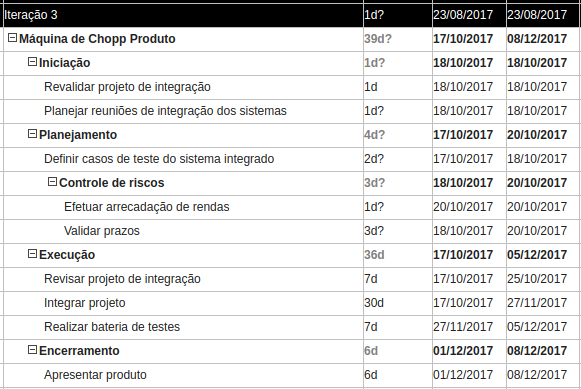
\includegraphics[scale= 0.7]{figuras/cronograma.png}
    \caption{Cronograma para a fase de integração de subsistemas. Fonte: Própria.}
    \label{cronograma}
\end{figure}